\documentclass[12pt]{article}
\usepackage{epsf,epic,eepic,eepicemu}
%\documentstyle[epsf,epic,eepic,eepicemu]{article}
\usepackage[utf8]{inputenc}
%\usepackage{amsmath}

\usepackage{wrapfig}
\usepackage{comment}
\usepackage{float}

\usepackage{graphicx}
\usepackage{subfig}



\begin{document}
%\oddsidemargin=-5mm \evensidemargin=-5mm \marginparwidth=.08in
%\marginparsep=.01in \marginparpush=5pt \topmargin=-15mm
%\headheight=12pt \headsep=25pt \footheight=12pt \footskip=30pt
%\textheight=25cm \textwidth=17cm \columnsep=2mm \columnseprule=1pt
%\parindent=15pt\parskip=2pt

\begin{center}
\bf Semestralní projekt MI-PAR 2010/2011:\\[5mm]
    Paralelní algoritmus pro řešení problému\\[5mm]
    Jeskyně pokladů\\[5mm]
       Ondřej Průcha\\
       Jakub Holý\\[2mm]
magisterské studium, FIT ČVUT, Kolejní 550/2, 160 00 Praha 6\\[2mm]
\today
\end{center}

\section{Definice problému}

\subsection{Vstupní data}

n = přirozené číslo představující počet předmětů \\
C[1..n] = reálné pole reprezentující ceny jednotlivých předmětů, 0.9  $\leq$ C[i] $\leq$ 1.1 \\
O[1..n] = reálné pole reprezentující objemy jednotlivých předmětů, 0.9 $\leq$ O[i] $\leq$ 1.1 \\
V = reálné číslo představující maximální objem předmetů, co lze odnést.

\subsection{Úkol}

Náhodou se shodou příznivých okolností ocitnete v jeskyni pokladů. Je zde mnoho (přesněji n) předmetů. U každého předmetu znáte jeho cenu a objem. Chcete si z této jeskyně odnést předměty v co největší celkové hodnotě, předměty ale můžete odnést jen ve svém batohu. Máte batoh, kam se vejde neomezený počet předmetů, ale má maximální objem V.

\subsection{Odchylky od zadání}

Z důvodu použitého algoritmu nebylo efektivní pracovat s čísly v plném desetinném rozvoji, tudíž jsme do algoritmu přidali možnost zvolení počtu platných desetinných míst.

\section{Popis sekvenčního algoritmu}

Použili jsme algoritmus z dynamického programování, který má za úkol řešit problém batohu (O/1 Knapsack problem).\\
\\
Na začátku algoritmu nastavíme počet předmětů, které máme k dispozici na nulu. Dále zvolíme velikost batohu 0, a poté ji postupně zvyšujeme podle zvolené přesnosti. Vzhledem k tomu, že zatím nemáme k dispozici žádné předměty, bude maximální dosažitelná cena rovna nule pro jakoukoli velikost batohu. Tuto část algoritmu skončime ve chvíli, kdy dosáhneme velikosti batohu podle zadání.\\

V každém dalším kroku přidáme mezi předměty, které máme k dispozici nový předmět. Nastavíme velikost batohu na 0, a pokračujeme stejně jako v předchozím kroku. Pokud zjistíme, že se nám tento nově přidaný předmět do batohu vejde, zkontrolujeme cenu dosaženou v predchozím kroku a pokud je cena vyšší, přidáme tento předmět do batohu a zapamatujeme si nově získanou maximální cenu.\\

Takto postupujeme tak dlouho, dokud nepřidáme všechny předměty. Výsledek pak na konci vyčteme z tabulky, ve které si pamatujeme, který předmět se nám vyplatil vzít při které velikosti batohu.

\section{Popis paralelního algoritmu a jeho implementace v MPI}

Každý proces v naší implementaci paralelního algoritmu pracuje na problému s jedním novým předmětem.\\
První proces začíná počítat úkol jeskyně s prvním předmětem a ostatní procesy čekají, dokud není k dispozici část výsledku prvního procesu. Každý předmět počítáme pro postupně se zvyšující kapacitu batohu a proto můžeme výsledek rozdělit podle kapacity batohu. Ve chvili, kdy je spočítána první část, jsou data odeslána druhému procesu a ten začíná počítat podle výsledků, které mu byly odeslány. Takto to platí až po počet procesorů. Ve chvíli, kdy první proces dokončí práci - to znamená, že se dopočítal do kapacity batohu podle zadání - započne práci na dalším předmětu pomocí odeslaných dat spočítaných posledním procesem. Pokud dojdou předměty, čekáme, až se poslední proces dopočítá do žádané kapacity batohu a pak lze výsledek jednoduše vyčíst stejným způsobem, jako u sekvenčního algoritmu. \\
\\
Program lze škálovat pomocí dvou zvolenych konstant. Pomocí první určujeme přesnost počítání podle desetinných míst a druhou konstantou nastavujeme velikost práce, kterou každý proces musí udělat, než odešle částečné výsledky dalšímu procesu na zpracování. Čím vyšší tuto konstantu zvolíme, tím menší budou nároky na komunikaci mezi procesy, ale procesy budou muset delší dobu čekat, než mohou začít pracovat.
\\
\\
\begin{comment}
	Job 35 inf	Job 35 eth	Job 40 inf	Job 40 eth	Job 45 inf	Job 45 eth
1	739	739	1020	1020	1322	1322
2	583	756	704	1148	976	1596
4	295	459	424	643	592	869
8	182	437	266	577	330	769
16	146	304	179	463	217	719
24	102	350	137	434	183	689
32	88	363	121	489	171	665
\end{comment}

Výsledný program potřebuje ke svému běhu pouze jeden parametr, a to cestu k souboru se zadáním. Soubor se zadáním má velmi jednoduchou strukturu: Jsou to čísla za sebou, kde první z nich je velikost batohu (reálné číslo), následuje počet prvků v batohu (celé číslo), a potom správný počet dvojic reálných čísel, kde první z dvojice je Cenou daného prvku, a druhé jeho Objemem. Po načtení udaného počtu prvků načítání končí a program začíná počítat. Jsou-li potom v zadávacím souboru nějaké další znaky, jsou ignorovány.

\section{Naměřené výsledky a vyhodnocení}

Měrili jsme 3 instance problému, kde jsme škálovali velikost batohu a počet výpočetních vláken. Zvolené velikosti byly 35, 40 a 45, při sto prvcích v ``jeskyni''. Každá instance byla měřena na 2, 4, 8, 16, 24 a 32 výpočetních jednotkách, které spolu komunikovaly přes Ethernet a pak přes InfiniBand.\\
\\
Na následujících grafech jsou znázorněny absolutní časy v sekundách, pro jednotlivé instance problému.

\begin{figure}[H]
\begin{center}
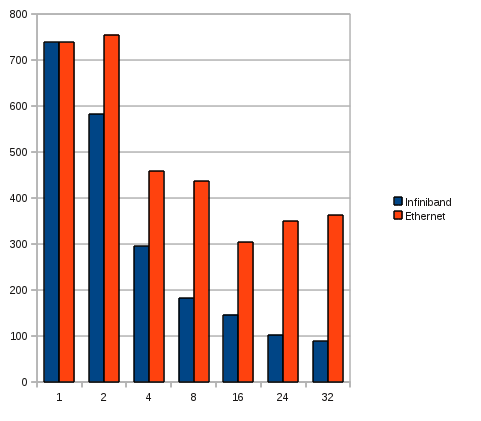
\includegraphics[width=0.6\textwidth]{par/35}
\caption{Graf časů výpočtu - batoh o velikosti 35}
\label{fig:problem_35}
\end{center}
\end{figure}

\begin{figure}[H]
\begin{center}
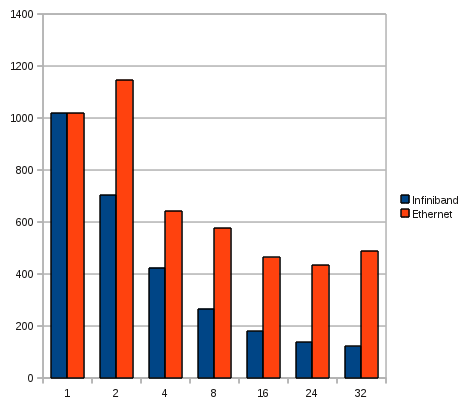
\includegraphics[width=0.6\textwidth]{par/40}
\caption{Graf časů výpočtu - batoh o velikosti 40}
\label{fig:problem_40}
\end{center}
\end{figure}

\begin{figure}[H]
\begin{center}
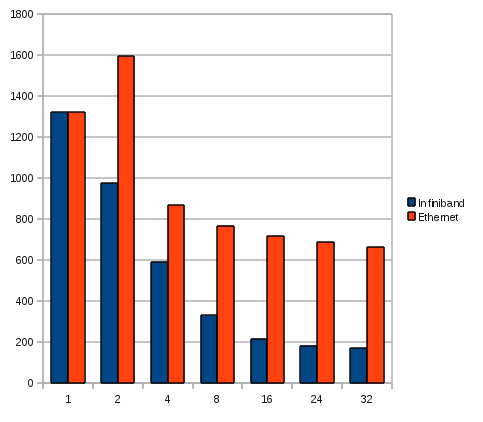
\includegraphics[width=0.6\textwidth]{par/45}
\caption{Graf časů výpočtu -  batoh o velikosti 45}
\label{fig:problem_45}
\end{center}
\end{figure}

Na těchto třech grafech je nezvykle vysoký čas výpočtu pro dvě jádra při použití komunikační sítě Ethernet - to je způsobeno relativně velkou zátěží způsobenou posíláním mezidat. Ve výsledku tedy přidání jedné jediné výpočetní jednotky znamená spíše zpomalení než zrychlení.\\
\\

Ze všech těchto údajů byly vytvořeny grafy zrychlení, diskuze následuje pod nimi:

\begin{figure}[H]
\begin{center}
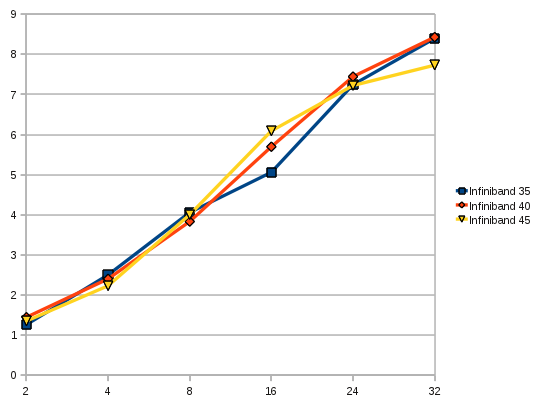
\includegraphics[width=0.6\textwidth]{par/inf}
\caption{Graf zrychlení při použití sítě InfiniBand}
\label{fig:inf}
\end{center}
\end{figure}

\begin{figure}[H]
\begin{center}
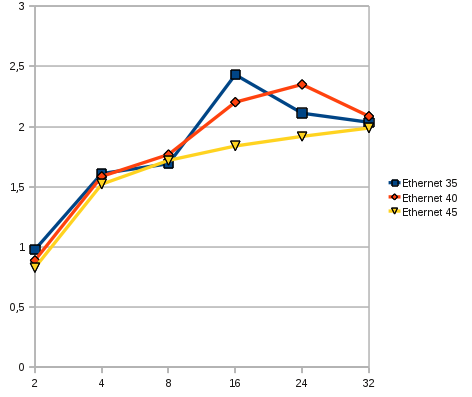
\includegraphics[width=0.6\textwidth]{par/eth}
\caption{Graf zrychlení při použití sítě Ethernet}
\label{fig:eth}
\end{center}
\end{figure}

Zvolené řešení zřetelně využívá komunikační síť, je tedy velmi náročné na přenosovou rychlost a odezvu mezi jednotlivýmí výpočetními jednotkami, což u sítě InfiniBand stále není problémem, narozdíl od (pomalejšího) Ethernetu. Z grafu lze vyčíst, že přidání výpočetních jednotek spojených sítí InfiniBand pokaždé o trochu zrychlilo výpočet. Výpočetní jednotky spojené sítí Ethernet však díky své rychlosti nebyly pokaždé zrychleny díky množství - v závislosti na složitosti problému bylo 24 nebo 32 výpočetních jednotek spíše důvodem zpomalení než zrychlení.\\
\\
Implementace by šla interně zlepšit pamatováním si poslední mezihodnoty změny (vlastně taková cache). Bez tohoto zapamatování pokaždé procházíme spojový seznam, což je lineárně složité samo o sobě. Algoritmus by šel škálovat změnou konstant zmíněných v odstavci o paralelním algoritmu, bylo by možné je předat jako parametr.\\
\\
%Granularita - stupeň paralelismu pro danou velikost řešeného problému

\section{Závěr}

Semestrální práce byla přínosná hned v několika ohledech - procvičení jazyka C/C++, seznámení se s paralelním prostředím, vytvoření reálné paralelní aplikace, seznámení s knihovnou MPI. Tyto znalosti jistě budou v blízké době velice užitečné (\#operationpayback).

\end{document}
